\documentclass[10.5pt,a4paper]{article}
\usepackage[margin=2cm,top=1.8cm,bottom=1.8cm]{geometry}
\usepackage{amsmath,amssymb}
\usepackage{graphicx}
\usepackage{booktabs}
\usepackage[table]{xcolor}
\usepackage{microtype}
\usepackage{caption}
\usepackage{enumitem}
\usepackage[colorlinks=true,linkcolor=blue!50!black,citecolor=green!40!black,urlcolor=blue!60!black]{hyperref}
\captionsetup{font=small,labelfont=bf}
\setlist{itemsep=1pt,topsep=3pt}
\graphicspath{{../figures/}}
\newcommand{\sq}{\sqrt{f}}
\newcommand{\dd}{\mathrm{d}}
\definecolor{idea}{RGB}{42,120,214}
\newcommand{\idea}[1]{\par\smallskip\noindent\colorbox{idea!8}{\parbox{\dimexpr\linewidth-2\fboxsep}{\small\textbf{\color{idea}Result.} #1}}\par\smallskip}

\title{\vspace{-8mm}\textbf{Radial ($\ell=0$) and dipole ($\ell=1$) oscillations of a static thin shell}\\[3pt]
\large Does the shell oscillate or collapse?}
\author{Juan Pablo Elia\\ \small GW\&AI Course}
\date{September 2026}

\begin{document}
\maketitle
\vspace{-5mm}

\begin{abstract}\noindent
A thin spherical shell of perfect fluid, with a flat interior and a Schwarzschild exterior of mass $M$, can sit at
rest at any radius $R>2M$ if its surface pressure is $p=\sigma(1-\sq)/4\sq$, $f=1-2M/R$. Its non-radial ($\ell\ge2$)
oscillations are known to contain a growing mode. Here we answer the complementary question: what happens to the
lowest multipoles, the radial ($\ell=0$) and dipole ($\ell=1$) oscillations of the shell itself? They do not radiate, so
they are true normal modes with real $\omega^2$, and their sign decides between oscillation and runaway. With
$x\equiv\sq$ and the adiabatic index $\Gamma$ of the surface fluid we find, in closed form,
\[
\frac{\omega_0^2R^3}{M}=\frac{2f}{1+\sq}\,\big(\Gamma-\Gamma_1\big),\quad \Gamma_1=\frac{1+2\sq+3f}{4f};\qquad
\frac{\omega_1^2R^3}{M}=\frac{6f}{1+3\sq}\,\big(\Gamma-\Gamma_{\rm dip}\big),\quad \Gamma_{\rm dip}=\Gamma_1-\frac1{6f},
\]
plus a zero-frequency dipole mode (rigid translation). The odd dipole has no oscillation at all: it is a slow rigid
rotation that drags the interior. For the equation of state used for this shell, $\Gamma=2$, the shell is radially
unstable for $R<3.82M$ and dipole unstable for $R<2.77M$; below $R=2.37M$ no causal equation of state can make it
radially stable. Following the unstable radial mode nonlinearly shows the shell collapsing to a black hole, the
thin-shell version of the classic gravitational collapse problem. Units $G=c=1$, time dependence $e^{-i\omega t}$,
$\omega$ measured in exterior (Schwarzschild) time.
\end{abstract}

\section{The question and why $\ell=0,1$ are special}
The shell sits at areal radius $R$. Inside, $\dd s^2=-\dd T^2+\dd r^2+r^2\dd\Omega^2$; outside,
$\dd s^2=-f\,\dd t^2+f^{-1}\dd r^2+r^2\dd\Omega^2$. The shell carries the surface stress tensor
$S_{ab}=(\sigma+p)u_au_b+p\,h_{ab}$ of a two-dimensional perfect fluid. The Israel junction conditions
\cite{Israel66,Poisson04}
\begin{equation}
[h_{ab}]=0,\qquad [K_{ab}]-h_{ab}[K]=-8\pi S_{ab}
\label{eq:israel}
\end{equation}
fix the static configuration (Poisson \cite{Poisson04}, Eqs.~3.80--3.81; Ipser \& Sikivie \cite{IS84}, Eqs.~3.7--3.9):
\begin{equation}
\sigma=\frac{1-\sq}{4\pi R},\qquad p=\kappa\sigma,\qquad \kappa=\frac{1-\sq}{4\sq}.
\label{eq:bg}
\end{equation}
A perturbation of the fluid needs an equation of state. We use the one of Pitre, Schneider \& Poisson \cite{PSP26}:
$\Gamma=\partial\ln p/\partial\ln\mu$ at fixed entropy, with $\mu$ the rest-mass surface density. The first law
$\dd\sigma=(\sigma+p)\,\dd\mu/\mu$ then gives the sound speed
\begin{equation}
v_s^2=\frac{\dd p}{\dd\sigma}=\frac{\Gamma p}{\sigma+p}=\frac{\Gamma\kappa}{1+\kappa},\qquad
\text{causality } (v_s\le1):\ \ \Gamma\le\Gamma_{\rm caus}=\frac{1+3\sq}{1-\sq}.
\label{eq:eos}
\end{equation}

\paragraph{What is different at $\ell=0,1$.} For $\ell\ge2$ the shell's oscillations couple to gravitational waves, and
the problem is a scattering or quasinormal-mode problem with complex frequencies. That problem has four matter modes per
$\ell$, one of them growing \cite{PSP26}. For $\ell=0$ and $\ell=1$ there is no radiation:
\begin{itemize}
\item $\ell=0$: by Birkhoff's theorem the exterior stays Schwarzschild. The only non-gauge vacuum perturbation is a
change $\delta M$ of the mass, which is static.
\item $\ell=1$, even: every vacuum perturbation is pure gauge, both in flat space and in Schwarzschild (Martel \& Poisson
\cite{MP05}, Sec.~IV\,D). Physically this is momentum conservation: the centre of mass cannot oscillate.
\item $\ell=1$, odd: the only non-gauge vacuum perturbation is a change $\delta J$ of the angular momentum (linearized
Kerr), which is static (\cite{MP05}, Sec.~V\,E).
\end{itemize}
The whole dynamics is therefore in the shell's matter and position, the frequencies are real or purely imaginary, and
$\omega^2$ is real: $\omega^2>0$ is an oscillation, $\omega^2<0$ an exponential runaway.

\section{Radial oscillations, $\ell=0$: exact equation of motion}
\idea{The radial problem can be solved exactly: the spherical shell moves in a one-dimensional effective potential.}

For a spherical shell $r=R(\tau)$, with $\tau$ its proper time, Eq.~\eqref{eq:israel} gives
$\sigma=[\sqrt{1+\dot R^2}-\sqrt{f(R)+\dot R^2}]/4\pi R$ \cite{IS84}. The conservation law $D_bS^{ab}=0$ is the first law
$\dd(\sigma A)+p\,\dd A=0$ with $A=4\pi R^2$, so $\dd\sigma/\dd R=-2(\sigma+p)/R$. With $m(R)\equiv4\pi R^2\sigma(R)$, write
$\alpha=\sqrt{1+\dot R^2}$ and $\beta=\sqrt{f+\dot R^2}$. Then $\alpha-\beta=m/R$ and $\alpha^2-\beta^2=2M/R$, so
$\alpha=M/m+m/2R$ and
\begin{equation}
\dot R^2+V(R)=0,\qquad V(R)=1-\Big(\frac Mm+\frac m{2R}\Big)^2 .
\label{eq:V}
\end{equation}
This is exact (nonlinear). A static shell sits where $V=V'=0$. Small displacements obey
$\delta\ddot R=-\tfrac12V''\,\delta R$. Using $m'=-8\pi Rp$ and $m''=-8\pi p+16\pi v_s^2(\sigma+p)$, and converting to
exterior time ($\dd\tau=\sq\,\dd t$ for a static shell), we get
\begin{equation}
\boxed{\ \frac{\omega_0^2R^3}{M}=\frac{4\Gamma f-3f-2\sq-1}{2(1+\sq)}=\frac{2f}{1+\sq}\,\big(\Gamma-\Gamma_1\big),\qquad
\Gamma_1=\frac{1+2\sq+3f}{4f}=\frac32+4\kappa+4\kappa^2\ }
\label{eq:w0}
\end{equation}
(\texttt{code/l0\_potential.py}). The shell is radially stable if and only if $\Gamma>\Gamma_1(R)$.
\begin{itemize}
\item The marginal index $\Gamma_1$ coincides \emph{identically} with the turning point of the equilibrium sequence,
$\dd M/\dd\mu=0$, of \cite{PSP26} (their Eq.~3.16) and LeMaitre \& Poisson \cite{LP19}. Those works gave the
stability criterion. Equation~\eqref{eq:w0} gives the actual frequency and growth rate.
\item Newtonian limit ($C=M/R\to0$): $\omega_0^2R^3/M=\Gamma-\tfrac32+\big(\tfrac54-\tfrac32\Gamma\big)C+O(C^2)$. The
leading term is the Newtonian result $\Gamma-3/2$ \cite{PSP26}. General relativity raises the required stiffness,
exactly as for stars.
\item \textbf{For $\Gamma=2$ the shell is radially unstable for $R<3.8165M$} ($C>0.2620$). This includes the compact
shells $R=2.2M$, $2.5M$ and $3M$ used for the trapped modes and echoes of this system.
\item $\Gamma_1$ exceeds the causal bound $\Gamma_{\rm caus}$ of Eq.~\eqref{eq:eos} for $R<2.370M$. There, \emph{no causal
equation of state can make the shell radially stable}. At the energy-condition limit $R=25M/12$, $\Gamma_1=9.5$.
\end{itemize}

\section{Dipole oscillations, $\ell=1$}
\subsection{Even parity: derivation from the Israel equations}
\idea{Because even $\ell=1$ vacuum perturbations are pure gauge, the metric can be left unperturbed on both sides. All
the physics is in how the shell is embedded in each side and in how its fluid moves.}

On each side we use coordinates in which the metric is exactly the background one. The gauge transformations of the two
sides are independent, and they are absorbed in the two embeddings. With intrinsic coordinates $y^a=(\tau,\theta,\phi)$,
$Y=\cos\theta$, and all amplitudes $\propto e^{-i\Omega\tau}$,
\begin{equation}
t_\pm=\frac{\tau}{\sqrt{F_\pm}}+\epsilon A_\pm Y,\qquad r_\pm=R+\epsilon X_\pm Y,\qquad
\theta_\pm=\theta+\epsilon B_\pm\,\partial_\theta Y,
\label{eq:emb}
\end{equation}
with $F_-=1$ inside and $F_+=f$ outside. The fluid has $\sigma\to\sigma+\epsilon sY$, $p\to p+\epsilon v_s^2sY$ and a
tangential velocity $u^\theta=\epsilon w\,\partial_\theta Y$. From Eq.~\eqref{eq:emb} we compute, on each side, the
induced metric and the extrinsic curvature
$K_{ab}=-n_\mu(\partial_be^\mu_a+\Gamma^\mu_{\nu\rho}e^\nu_ae^\rho_b)$ to first order. Then we impose
Eq.~\eqref{eq:israel}: continuity of $h_{ab}$ and the Israel equations, for the $\tau\tau$, $\tau\theta$,
$\theta\theta$ and $\phi\phi$ components (\texttt{code/israel\_low\_l.py}, SymPy). A reparametrization of the shell
$y^a\to y^a+\epsilon\zeta^a$ shifts $A_\pm$ and $B_\pm$ together. We fix it with $A_-=B_-=0$ and have checked that
fixing it on the exterior side instead gives identical frequencies. This leaves six unknowns,
$(X_-,A_+,X_+,B_+,s,w)$, and six independent equations. The zeroth order of every equation vanishes for the
background~\eqref{eq:bg}.

The same code with $Y=1$ solves the $\ell=0$ problem. It reproduces Eq.~\eqref{eq:w0} identically, an independent check
of the whole construction (normal, curvature, fluid terms). For $\ell=1$ the determinant is
\begin{equation}
\det\propto\Omega^2\Big[\,4\Omega^2x^2(3x+1)+12\Gamma x^2(x^2-1)-9x^4-6x^3+8x^2+6x+1\Big],\qquad x=\sq,
\end{equation}
which gives, with $\omega=\sq\,\Omega$,
\begin{equation}
\boxed{\ \frac{\omega_1^2R^3}{M}=\frac{12\Gamma f-9f-6\sq-1}{2(1+3\sq)}=\frac{6f}{1+3\sq}\,\big(\Gamma-\Gamma_{\rm dip}\big),
\qquad \Gamma_{\rm dip}=\frac{(1+3\sq)^2}{12f}=\Gamma_1-\frac1{6f}\ }
\label{eq:w1}
\end{equation}
and a double root $\Omega=0$.
\begin{itemize}
\item \textbf{Zero mode.} Its null vector is $X_-=-RB_+$, with $X_+=s=w=0$: the shell is \emph{rigidly translated}
relative to the interior flat space and stays centred in the exterior. The double root corresponds to the translation
and the uniform motion (boost). This is the relativistic version of the zero mode found by \cite{PSP26}
(their Eq.~10.58).
\item \textbf{Oscillating mode.} The shell's geometric centre moves while its surface density develops a dipole
(Fig.~\ref{fig:pattern}). The centre of mass stays fixed: in the Newtonian limit the eigenvector satisfies
$X_++sR/3\sigma=0$, with a residual that vanishes as $M/R$. The restoring force is the pressure of the compressed side.
\item Newtonian limit: $\omega_1^2R^3/M\to\tfrac12(3\Gamma-4)$, exactly Eq.~10.57 of \cite{PSP26}. It also matches our own
Newtonian shell equations evaluated at $\ell=1$ (\texttt{code/check\_newtonian.py}). Relativistic correction:
$+\big(\tfrac32-\tfrac{15}8\Gamma\big)C$.
\item Since $\Gamma_{\rm dip}<\Gamma_1$ at every radius, \textbf{a radially stable shell is always dipole stable}. For
$\Gamma=2$ the dipole mode is unstable only for $R<2.767M$. A causal equation of state can stabilize it down to
$R=9M/4$ exactly.
\end{itemize}

\begin{figure}[t]\centering
\begin{minipage}{0.49\textwidth}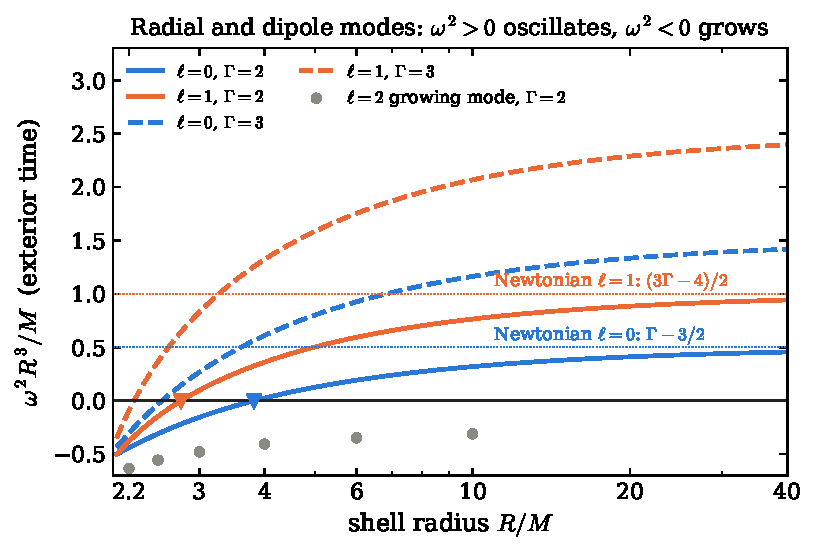
\includegraphics[width=\linewidth]{l01_f1_omega2.pdf}
\caption{$\omega^2R^3/M$ of the radial (blue) and dipole (orange) modes for $\Gamma=2$ (solid) and $\Gamma=3$ (dashed).
Triangles: marginal radii for $\Gamma=2$. Grey: the growing $\ell=2$ matter mode, $-({\rm Im}\,\omega)^2R^3/M$.
Dotted: Newtonian limits.}\label{fig:w2}\end{minipage}\hfill
\begin{minipage}{0.49\textwidth}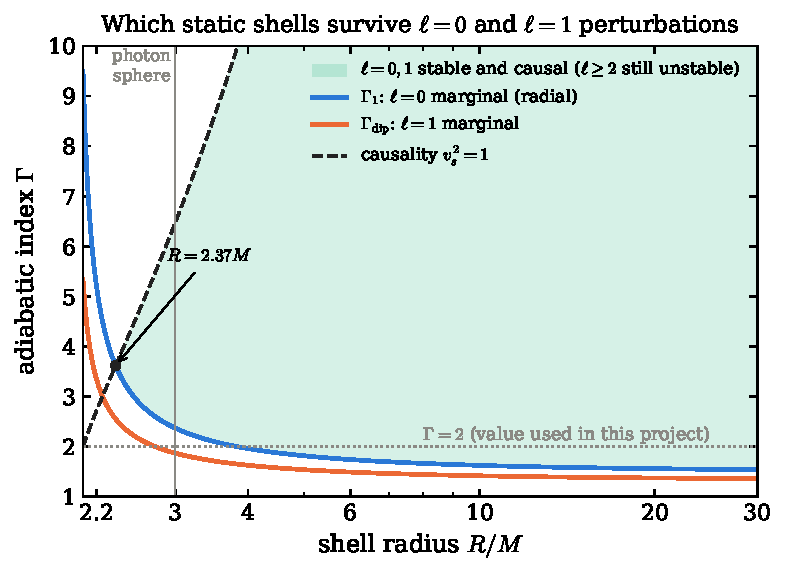
\includegraphics[width=\linewidth]{l01_f2_stability.pdf}
\caption{Stability in the $(R,\Gamma)$ plane. Above $\Gamma_1$: radially stable; above $\Gamma_{\rm dip}$: dipole stable;
below the dashed line: causal. Shaded: stable against $\ell=0,1$ with a causal equation of state.}\label{fig:stab}\end{minipage}
\end{figure}

\subsection{Odd parity: no oscillation, only rotation}
For odd parity the conservation law $D_bS^{ab}=0$ gives $\partial_\tau u_A=0$ at every $\ell$. The shell's matter
cannot oscillate axially, so there is \emph{no odd matter mode at any $\ell$}, and no odd dipole oscillation. The only odd
$\ell=1$ solution is stationary: a slow rigid rotation. Outside, $g_{t\phi}=-(2J/r)\sin^2\theta$. Inside, the flat
space rotates rigidly. Continuity of $h_{\tau\phi}$ and the $\tau\phi$ Israel equation give
(\texttt{code/l1\_odd\_rotation.py})
\begin{equation}
\Omega_{\rm drag}=\frac{2J}{R^3},\qquad \frac{\Omega_{\rm drag}}{\Omega_{\rm shell}}=\frac{(1-\sq)(1+3\sq)}{1+2\sq}
\ \xrightarrow{\ M/R\to0\ }\ \frac{4M}{3R},\qquad \xrightarrow{\ R\to2M\ }\ 1 .
\end{equation}
Here $\Omega_{\rm drag}$ is the angular velocity at which the interior's local inertial frames rotate and
$\Omega_{\rm shell}$ that of the fluid, both in exterior time. The weak-field limit is Thirring's classic frame-dragging
result \cite{Thirring18}. The limit $R\to2M$ is complete dragging, as found by Brill \& Cohen \cite{BrillCohen66}. The same
equation returns $J=\frac{8\pi}3R^2(\sigma+p)U$, the shell's own angular momentum.

\begin{figure}[t]\centering
\begin{minipage}{0.49\textwidth}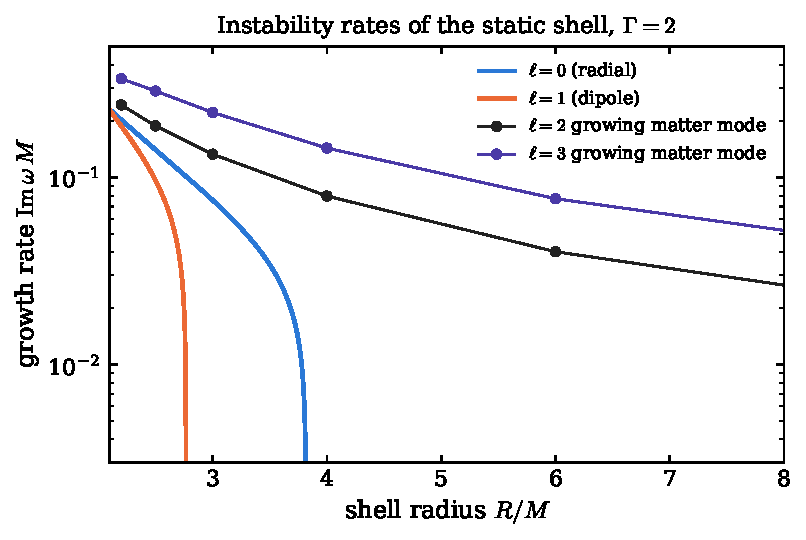
\includegraphics[width=\linewidth]{l01_f3_rates.pdf}
\caption{Growth rates for $\Gamma=2$: radial and dipole (this work) and the growing $\ell=2,3$ matter modes of the same
shell.}\label{fig:rates}\end{minipage}\hfill
\begin{minipage}{0.49\textwidth}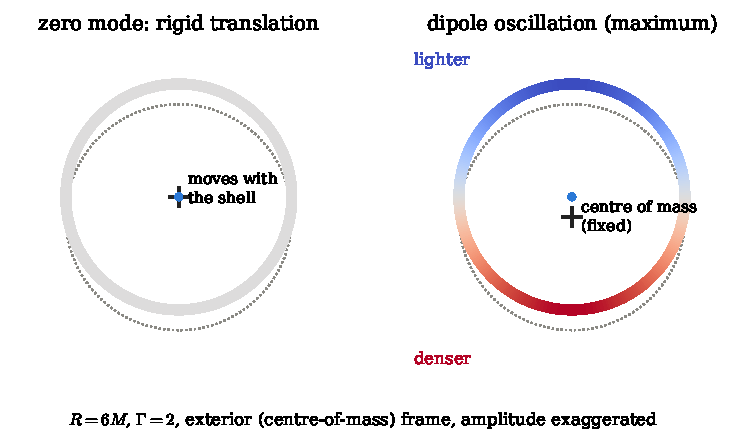
\includegraphics[width=\linewidth]{l01_f6_dipole_pattern.pdf}
\caption{The two even dipole modes. Left: zero mode (translation). Right: dipole oscillation, colour = surface
density; the centre of mass (cross) does not move.}\label{fig:pattern}\end{minipage}
\end{figure}

\begin{table}[h]\centering\small
\caption{Marginal indices and frequencies. $\Gamma_{\rm caus}$ is the largest causal $\Gamma$. $\omega M$ is real for an
oscillation and imaginary for a growing mode. Last column: the growing $\ell=2$ matter mode of the same shell, from the
full even-parity junction with radiation.}\label{tab:modes}
\begin{tabular}{rccc|cc|cc|c}\toprule
 & \multicolumn{3}{c|}{marginal / causal $\Gamma$} & \multicolumn{2}{c|}{$\ell=0$, $\Gamma=2$} & \multicolumn{2}{c|}{$\ell=1$, $\Gamma=2$} & $\ell=2$, $\Gamma=2$\\
$R/M$ & $\Gamma_1$ & $\Gamma_{\rm dip}$ & $\Gamma_{\rm caus}$ & $\omega^2R^3/M$ & $\omega M$ & $\omega^2R^3/M$ & $\omega M$ & $\omega M$ (growing)\\\midrule
2.2 & 5.158 & 3.325 & 2.73 & $-0.4412$ & $0.2036\,i$ & $-0.3795$ & $0.1888\,i$ & $0.2443\,i$ \\
2.5 & 3.118 & 2.285 & 4.24 & $-0.3090$ & $0.1406\,i$ & $-0.1459$ & $0.0966\,i$ & $0.1886\,i$ \\
3 & 2.366 & 1.866 & 6.46 & $-0.1547$ & $0.0757\,i$ & $+0.0981$ & $0.0603$ & $0.1332\,i$ \\
4 & 1.957 & 1.624 & 10.66 & $+0.0251$ & $0.0198$ & $+0.3616$ & $0.0752$ & $0.0796\,i$ \\
6 & 1.737 & 1.487 & 18.80 & $+0.1928$ & $0.0299$ & $+0.5944$ & $0.0525$ & $0.0401\,i$ \\
10 & 1.622 & 1.413 & 34.89 & $+0.3197$ & $0.0179$ & $+0.7647$ & $0.0277$ & $0.0176\,i$ \\
100 & 1.510 & 1.340 & 394.99 & $+0.4824$ & $0.0007$ & $+0.9774$ & $0.0010$ & -- \\
\bottomrule\end{tabular}

\end{table}

\section{Beyond linear order: the unstable shell collapses}
\idea{The exact potential~\eqref{eq:V} lets us follow the radial instability to the end. The unstable shell either
collapses through its horizon or makes a large bounded excursion. This is the thin-shell analogue of the collapse of a
spherical body \cite{LL}.}

To go nonlinear we need the full equation of state. We take a polytrope \cite{PSP26}, $p=K\mu^\Gamma$ and
$\sigma=\mu+p/(\Gamma-1)$, with rest-mass conservation $\mu\propto R^{-2}$, and choose $K$ so that the shell of
Eq.~\eqref{eq:bg} at $R_0$ is an equilibrium. The shell is released from rest at $R_0(1\pm\delta)$ and
$\ddot R=-V'/2$ is integrated (\texttt{code/l0\_nonlinear.py}; Figs.~\ref{fig:V}, \ref{fig:traj}).
\begin{itemize}
\item $R_0=6M$ (stable). The shell oscillates about $R_0$. The measured frequency, $\Omega=0.036579/M$ in proper time for
a 1\% amplitude, agrees with Eq.~\eqref{eq:w0} ($0.036588/M$) to $0.03\%$. $V$ has a barrier at $R\approx2.97M$, so a
large enough inward kick collapses even this shell.
\item $R_0=3M$, pushed inward by $10^{-3}$. The shell leaves its equilibrium exponentially (linear e-folding time $7.6M$)
and crosses $r=2M$, forming a black hole, after $\tau=45.6M$ of proper time. A distant observer sees it freeze at the
horizon.
\item $R_0=3M$, pushed outward. The shell does not escape. It is gravitationally bound: its rest mass exceeds $M$ by
$3.6\%$. It expands to $9.5M$, falls back, and lingers near the unstable equilibrium. Any further inward perturbation
there sends it into the black hole.
\end{itemize}

\begin{figure}[t]\centering
\begin{minipage}{0.49\textwidth}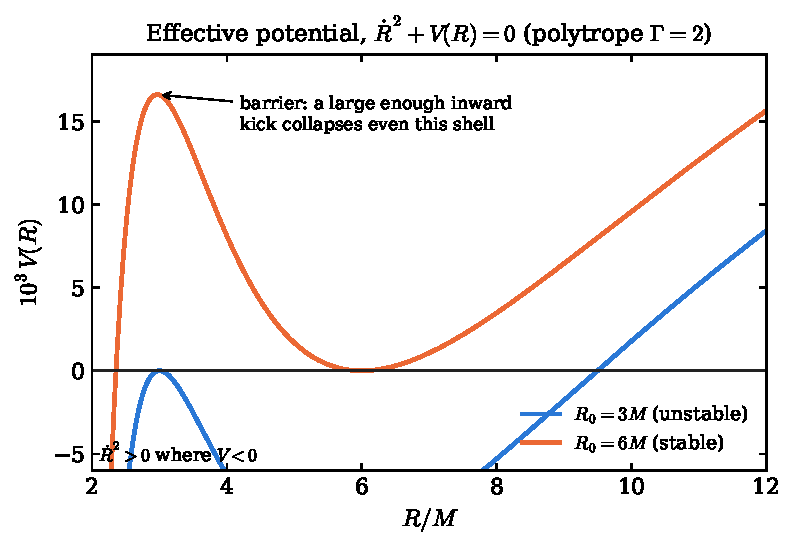
\includegraphics[width=\linewidth]{l01_f4_potential.pdf}
\caption{Exact effective potential~\eqref{eq:V} of a polytropic ($\Gamma=2$) shell in equilibrium at $3M$ (a maximum:
unstable) and $6M$ (a minimum: stable).}\label{fig:V}\end{minipage}\hfill
\begin{minipage}{0.49\textwidth}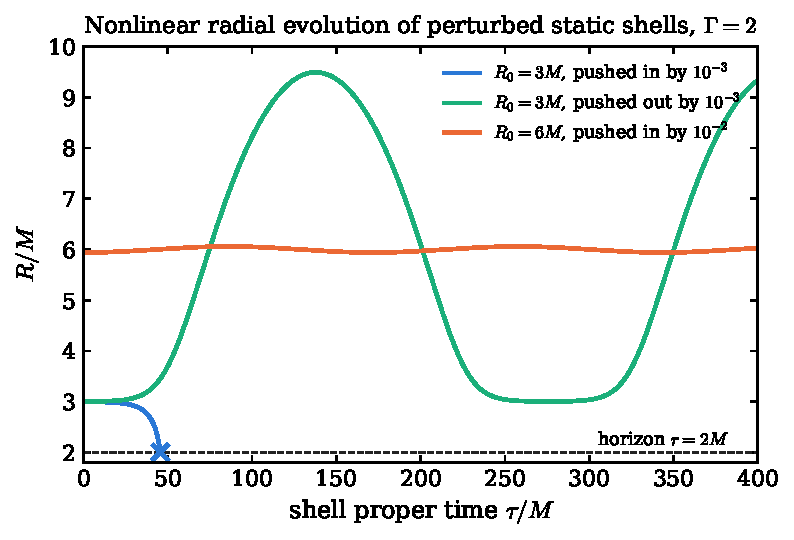
\includegraphics[width=\linewidth]{l01_f5_trajectories.pdf}
\caption{Nonlinear radial evolution. The unstable shell collapses through $r=2M$ (cross) or makes a large bounded
excursion; the stable one oscillates.}\label{fig:traj}\end{minipage}
\end{figure}

\section{How important are these modes compared with $\ell\ge2$?}
Figure~\ref{fig:rates} and Table~\ref{tab:modes} compare the growth rates for $\Gamma=2$.
\begin{itemize}
\item Wherever the radial mode is unstable, it grows somewhat more slowly than the $\ell=2$ matter mode: by a factor
$0.83$ at $2.2M$ and $0.57$ at $3M$. The time scale is the same, $(R^3/M)^{1/2}$, and is much longer than the wave periods
$\sim R$. The adiabatic picture of scattering off a static shell is therefore not changed.
\item The radial instability matters because of its outcome. An $\ell\ge2$ runaway deforms the shell. An $\ell=0$ runaway
is \emph{total collapse to a black hole}, or a large pulsation.
\item The $\ell\ge2$ instability is present for every $\Gamma$ \cite{PSP26}. The $\ell=0,1$ instabilities, by contrast,
disappear for a stiff enough causal fluid, but only if $R>2.37M$. The ultracompact shells that produce echoes
($R<3M$) therefore need $\Gamma$ between $\Gamma_1$ (2.4 to 3.6) and the causal limit to avoid collapse.
\end{itemize}

\section{Validation}
\begin{center}\small
\begin{tabular}{p{0.52\linewidth}p{0.42\linewidth}}\toprule
check & result\\\midrule
$\ell=0$: exact potential vs linearized Israel equations (two independent derivations) & identical (symbolic difference $0$)\\
$\ell=0$ marginal index vs turning point $\dd M/\dd\mu=0$ of \cite{PSP26,LP19} & identical\\
Newtonian limits: $\ell=0$, $\Gamma-\tfrac32$; $\ell=1$, $\tfrac12(3\Gamma-4)$ and $0$ & agree with \cite{PSP26} Sec.~10\,H and with our own Newtonian equations\\
background Israel equations at zeroth order (16 components) & all vanish\\
gauge fixing interior ($A_-=B_-=0$) vs exterior ($A_+=B_+=0$) & same frequencies\\
redundant components ($\phi\phi$, second angle) & add no rank (random numerical tests)\\
$\ell=1$ zero mode & rigid translation (as \cite{PSP26} Eq.~10.58)\\
$\ell=1$ oscillation: centre of mass fixed (Newtonian) & residual $\propto M/R$ ($5\times10^{-5}$ at $R=10^4M$)\\
nonlinear vs linear radial frequency ($R_0=6M$) & $0.03\%$\\
odd $\ell=1$: weak-field and $R\to2M$ limits of the frame dragging & $4M/3R$ (Thirring), $1$ (complete dragging)\\\bottomrule
\end{tabular}
\end{center}

\section{Conclusions}
\begin{enumerate}
\item The static fluid shell has one radial mode and, per $m$, one oscillating even dipole mode plus a translation zero
mode. Both have closed-form frequencies, Eqs.~\eqref{eq:w0} and~\eqref{eq:w1}. The odd dipole never oscillates; it is a
slow rotation that drags the interior.
\item Radial stability requires $\Gamma>\Gamma_1=(1+2\sq+3f)/4f$ and dipole stability $\Gamma>\Gamma_1-1/6f$, so the
radial mode is always the more dangerous one. For the $\Gamma=2$ shell the radial mode is unstable inside $3.82M$ and the
dipole inside $2.77M$. Inside $2.37M$ no causal fluid can hold the shell up against radial collapse.
\item The unstable radial mode is the onset of gravitational collapse. Followed nonlinearly, the shell falls through its
Schwarzschild radius in a few tens of $M$ of proper time, or rebounds as a large bounded pulsation.
\end{enumerate}

\noindent\colorbox{idea!8}{\parbox{\dimexpr\linewidth-2\fboxsep}{\small\textbf{\color{idea}Next step.} The natural
continuation is to put the $\ell\ge2$ gravitational perturbations on top of this collapsing background: first the odd
parity, whose junction is a $\delta$-barrier of strength $\sq(1-\sq)/R$ that can simply follow $R(\tau)$. This gives the
waveform emitted while the shell collapses, and shows how its ringing turns into black-hole ringing as the horizon
forms. It is the thin-shell analogue of the calculation of Cunningham, Price \& Moncrief \cite{CPM78} for a collapsing dust
ball.}}

\vspace{2mm}
{\footnotesize
\begin{thebibliography}{99}\setlength{\itemsep}{0pt}
\bibitem{Israel66} W.~Israel, Nuovo Cimento B \textbf{44}, 1 (1966).
\bibitem{Poisson04} E.~Poisson, \emph{A Relativist's Toolkit} (Cambridge University Press, 2004), Ch.~3.
\bibitem{IS84} J.~Ipser and P.~Sikivie, Phys.\ Rev.\ D \textbf{30}, 712 (1984).
\bibitem{MP05} K.~Martel and E.~Poisson, Phys.\ Rev.\ D \textbf{71}, 104003 (2005).
\bibitem{PSP26} T.~Pitre, B.~Schneider and E.~Poisson, Phys.\ Rev.\ D \textbf{113}, 124055 (2026), arXiv:2604.05980.
\bibitem{LP19} P.~LeMaitre and E.~Poisson, Am.\ J.\ Phys.\ \textbf{87}, 961 (2019).
\bibitem{Thirring18} H.~Thirring, Phys.\ Z.\ \textbf{19}, 33 (1918).
\bibitem{BrillCohen66} D.~R.~Brill and J.~M.~Cohen, Phys.\ Rev.\ \textbf{143}, 1011 (1966).
\bibitem{CPM78} C.~T.~Cunningham, R.~H.~Price and V.~Moncrief, Astrophys.\ J.\ \textbf{224}, 643 (1978).
\bibitem{LL} L.~D.~Landau and E.~M.~Lifshitz, \emph{The Classical Theory of Fields}, 4th ed.\ (Pergamon, 1975), sections on gravitational collapse.
\end{thebibliography}}
\end{document}
